\documentclass{article}
\usepackage{graphicx}
\usepackage{amsmath, amsfonts, mathtools}
\usepackage{amsthm}
\usepackage{todonotes}
\usepackage[ruled, linesnumbered]{algorithm2e}
\usepackage{enumerate}
\usepackage{float}
\usepackage{subcaption}
\usepackage{dsfont}
\usepackage{pythonhighlight}
\usepackage{listings}
\usepackage{xcolor}
\usepackage{xurl}

% Define colors for syntax highlighting
\definecolor{codegreen}{rgb}{0.2,0.6,0.2}
\definecolor{codegray}{rgb}{0.5,0.5,0.5}
\definecolor{codepurple}{rgb}{0.58,0,0.82}
\definecolor{backcolour}{rgb}{0.95,0.95,0.92}


% Sensible defaults for lstlistings
\lstset{
numberstyle=\tiny\color{codegray},
backgroundcolor=\color{backcolour},   
  basicstyle=\footnotesize\ttfamily,
  belowcaptionskip=1\baselineskip,
  breaklines=true,
  commentstyle=\bfseries\color{purple!40!black}
  frame=L,
  identifierstyle=\color{blue},
  keywordstyle=\bfseries\color{green!40!black},
  language=python,
  showstringspaces=false,
  stringstyle=\color{orange},
  xleftmargin=\parindent,
  captionpos=b,                    
    keepspaces=true,                 
    numbers=left,                    
    numbersep=5pt,                  
    showspaces=false,                
    showstringspaces=false,
    showtabs=false,
    tabsize=2,
    framexleftmargin=16pt,
    framextopmargin=6pt,
        framexbottommargin=6pt, 
        frame=tb, framerule=0pt,
}


\title{Approximation Algorithms - Assignment 3}
\author{Group 2: Christoph Kern, Johannes Gabriel Sindlinger}


\begin{document}

\maketitle

\section{Scheduling Jobs with Precedence Constraints}
We consider scheduling jobs on identical machines as in Section 2.3, but jobs are now subject to \emph{precedence constraints}. We say $i \prec j$ if in any feasible schedule, job $i$ must be completely processed before job $j$ begins processing. A natural variant on the list scheduling algorithm is one in which whenever a machine becomes idle, then any remaining job that is available is assigned to start processing on that machine. A job $j$ is available if all jobs $i$ such that $i \prec j$ have already been completely processed. Show that this list scheduling algorithm is a $2$-approximation algorithm for the problem with precedence constraints.

\begin{proof}
    Like in the original problem, following two lower bounds on the length of an optimal schedule $C^*_{\max}$ hold:
    \[
        C^*_{\max} \ge \max_{j=1,\dots,n}p_j
        \quad\quad\quad\quad
        C^*_{\max} \ge \sum^n_{j=1}\frac{p_j}{m}
    \]
    However, we can now define an additional lower bound. We observe that the precedence constraints form a directed acyclic graph $G$, where we have a vertex for each job and an edge from job $i$ to job $j$ iff $i \prec j$. Since for any path $P$ in $G$ any two jobs can not run simultaneously, we have
    \[
        C^*_{\max} \ge \sum_{i \in P} p_{i}
    \]

    
    However, we can now define an additional lower bound. Let $i_1,i_2, \dots, i_k$ be a set of jobs s.t.~$i_1 \prec i_2 \prec \dots \prec i_k$. Then,
    \[
        C^*_{\max} \ge \sum_{j = 1}^k p_{i_j}
    \]
    Let $\ell$ be a job that completes in the final schedule. The completion time of job $\ell$, $C_\ell$, is equal to this solution's objective function value. We now consider the start time $S_\ell = C_\ell - p_\ell$ of job $S_\ell$. We now distinguish between two cases:
    \begin{itemize}
        \item All machines are busy up to $S_\ell$:
        \item There is a machine $x$ not busy before $S_\ell$:
        \todo{wrong}
        
    \end{itemize}
\end{proof}

\section{Asymmetric TSP}

The Wikipedia article on TSP claims that it is possible to solve TSP in the setting where distances are asymmetric, by reducing this to the standard (symmetric) case. In the reduction some vertices that have "no edges" between them; you can think of this as having infinite (or very large) weight. Explain how to choose the value $w$ and argue that the reduction is correct.  Why does this reduction not imply a $\frac{3}{2}$-approximation for the asymmetric TSP?

\begin{proof}
    We aim to show that the reduction is correct. Let $G=(V,E)$ be the original complete graph ($|V| = n$) and $G'=(V',E')$ the reduced graph, such that
    \begin{align*}
        V' &= \{v_i, v_i'\ |\ v_i \in V\}\\
        E' &= V' \times V'
    \end{align*}
    This creates a mirrored set of vertices of the original vertices, which we refer to as ghost vertices (indicate by $'$). The vertices between an original vertex $v_i \in V'$ and its corresponding ghost vertex $v_i' \in V'$ will be referred to as a ghost edges. 

    The asymmetric weights $w_{v_i \to v_j}$ of $G$ will be mapped to symmetric weights in our constructed graph as follows:
    \[
        w_e = \begin{cases}
            w_{v_i \to v_j} & \text{if }e = (v_i', v_j)\\
            w & \text{if }e = (v_i, v_i')\\
            \infty & \text{otherwise}
        \end{cases} \text{ for every } e \in E'
    \]

    The weight $w$ of the ghost edges will be defined later in the reduction. Edges between two original vertices or between to ghost vertices will have infinite weight, as they are not supposed to be used.
    
    
    We claim that there exists a tour $C$ in $G$ such that $\text{cost}(C) \le d$ iff there exists a tour $C'$ in $G'$ such that $\text{cost}(C') \le d + n \cdot w$. We show the correctness of both directions of this equivalence relation.

    \begin{itemize}
        \item[$(\Rightarrow)$]  Let $C = v_1 \rightarrow v_2 \rightarrow \dots \rightarrow v_n \rightarrow v_1$ be a tour of $G$ such that $\text{cost}(C) \le d$. We can create an equivalent tour $C' = v_1 \rightarrow v_1' \rightarrow v_2\rightarrow v_2' \rightarrow \dots \rightarrow v_n \rightarrow v_n' \rightarrow v_1$ in $G'$, where every vertex $v_i \in V$ is simply replaced by the sequence $v_i \rightarrow v_i'$. Since every vertex must be part of the tour, also all ghost edges must be part of our constructed tour, which together adds a cost of $n \cdot w$. Since the remaining edges are equivalent to those of the original tour, also in terms of weight, we end up with \[cost(C') = cost(C) + n \cdot w \le d + n \cdot w.\]

        \item [$(\Leftarrow)$] Let $C'$ be some tour of $G'$ such that $\text{cost}(C') \le d + n \cdot w$. If $C'$ contains two consecutive original vertices or two consecutive ghost vertices, then $cost(C') = \infty$. As $w$ is not infinity, we have $d = \infty$. As any tour in $G$ will have a cost less than or equal to $\infty$, it will also have a cost less than $d$. 
        
        Now consider the case where we only have alternating original and ghost vertices. Furthermore, lets restrict ourselves to the case where all ghost edges are traversed by the tour. W.l.o.g.~suppose the tour starts at the original vertex $v_1$ and is followed by ghost vertex $v_1'$ (otherwise traverse the tour in the other direction; this must be equivalent in cost due to symmetry). Then the tour $C'$ must have following shape:
        \[
            C' = v_1 \rightarrow v_1' \rightarrow v_2'\rightarrow v_2' \rightarrow \dots \rightarrow v_n \rightarrow v_n' \rightarrow v_1
        \]
        
        We can then merge all regular vertices with its corresponding ghost vertex in the tour which results in a tour $C$ for $G$, where the edges have the same weight as in $C'$. Since $\text{cost}(C) = \text{cost}(C') - n \cdot w$, we have $\text{cost}(C) \le d$.

        Finally, suppose the tour $C'$ does not contain the ghost edge $(v_i, v_i')$. We will now show how to construct a tour $C''$ of $G$ from $C'$ which contains the ghost edge $(v_i, v_i')$ such that $\text{cost}(C'') \le \text{cost}(C')$. This procedure can then be applied for every ghost edge, which allows us to use the above construction for a tour $C$ in $G$, resulting in $\text{cost}(C) \le d$.

        \begin{figure}[]
            \centering
            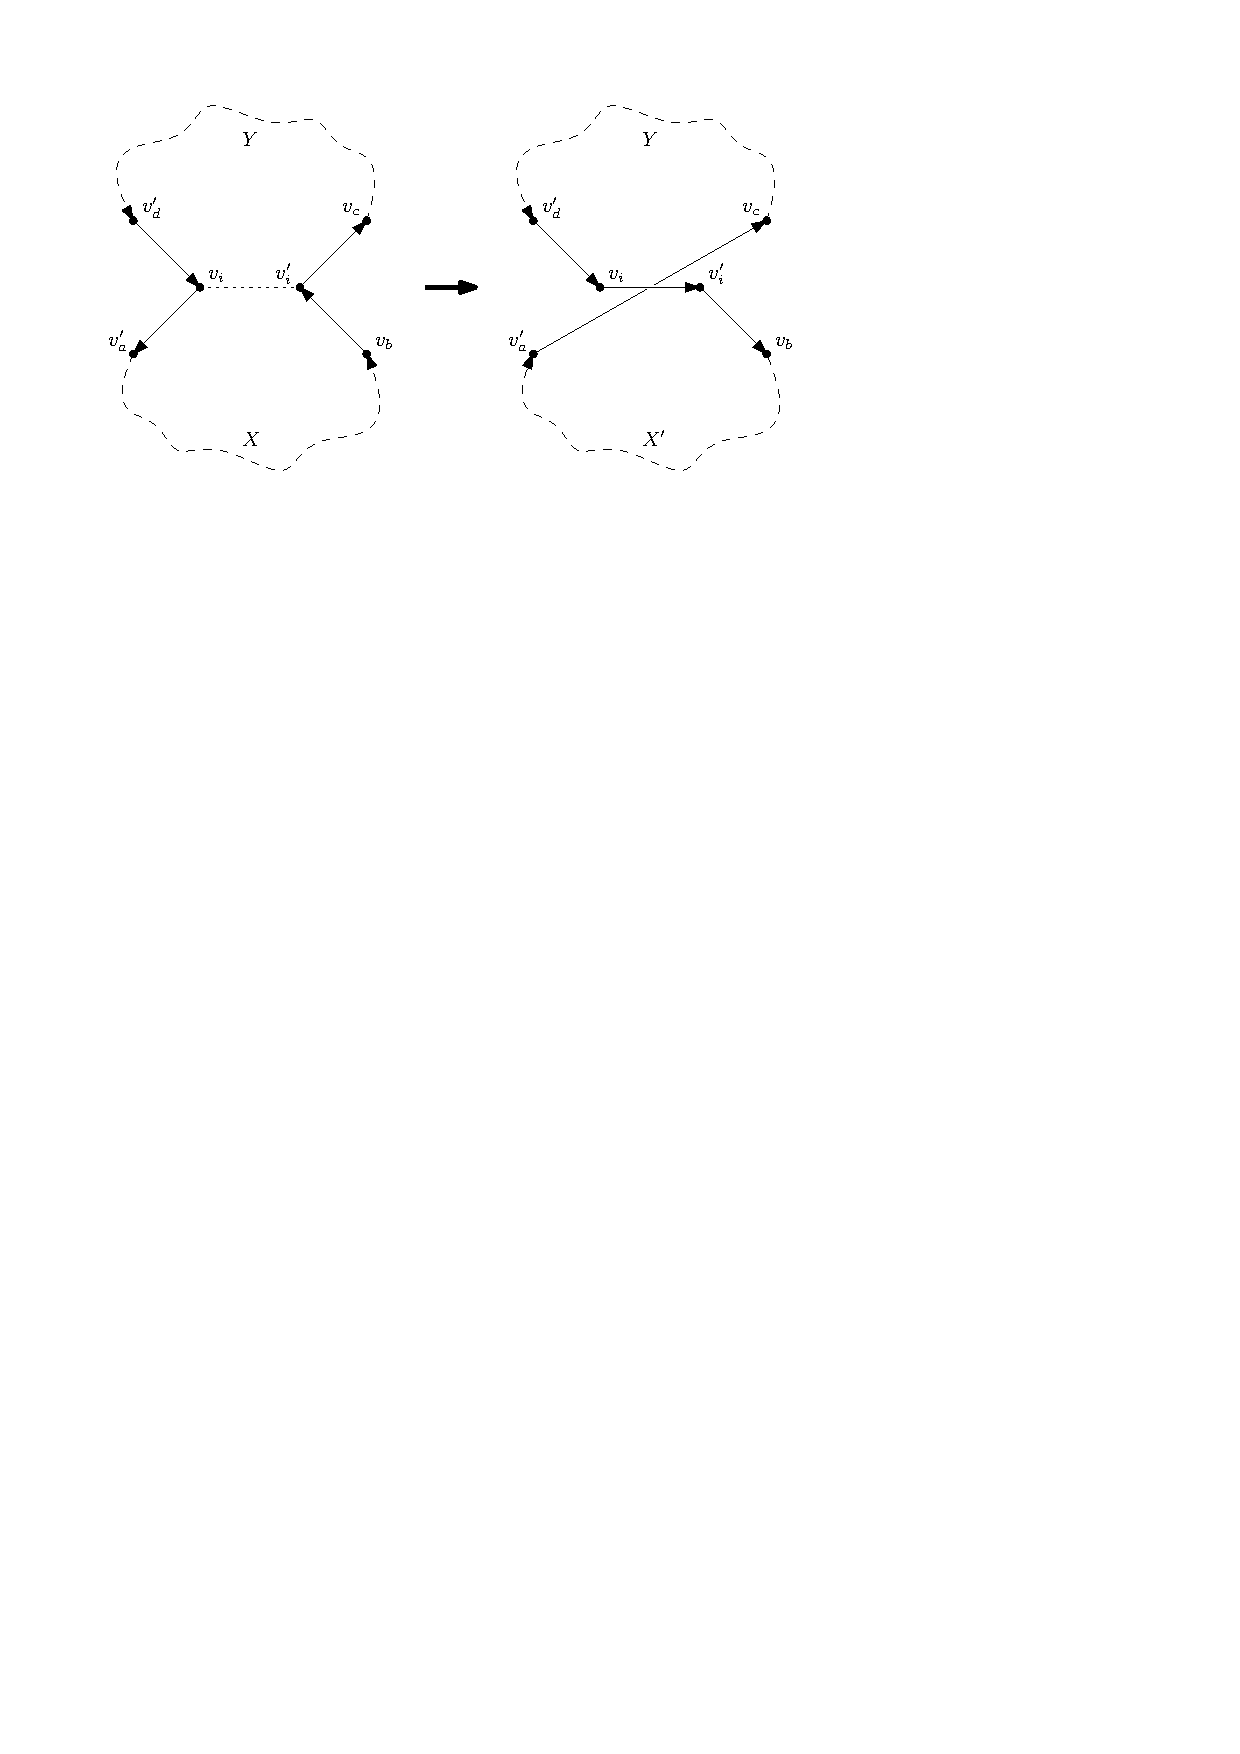
\includegraphics{Assignment3/figures.pdf}
            \caption{Caption}
            \label{fig:enter-label}
        \end{figure}

        

        
    \end{itemize}
    
   


\end{proof}
\end{document}
